\documentclass{article}
\usepackage{graphicx}
\usepackage{pdflscape}
\usepackage{rotating}
\title{Core Circuit Model }
\author{Joshua Resnick}
\setlength\parindent{0pt}
\begin{document}
\maketitle


The model is built up in the following way. The core is modeled as 4 delay segments with the same characteristic impedance (1.55 ohms in this case) and 3 resistors. The three resistors represent the heated and unheated parts of the core - the middle resistor represents the part of the core heated by the cartridge heater. The output transmission line is just a delay with an impedance, and the termination resistor is just an ideal resistor. The respective delays of the core and output line can be measured from the respective waveform, so these are not really a degree of freedom. If RCore1 to RCore3 are all set to be equal (i.e. not modelling the variability in resistance across the core) then RCoreTotal collapses to a single degree of freedom. Likewise, we can set the impedance parameter for Core1, Core2, and Core3 to be equal. This gives us the following 4 degrees of freedom:
CoreZ, RCore, OutputLineZ, and RTerm.

RCore and RTerm dominate the amplitude components of the output, so they can be independently tuned by matching waveform amplitudes. So, I think we are primarily dealing with CoreZ and OutputLineZ as the tune-able variables. 
The model has a 5 segment transmission line of "known" impedance of 1.55 ohms.

Each segment has a known transmission line delay (i.e. length at the speed of light in the transmission line).  Speed of light in the transmission line is determined by the relative dielectric constant of the substrate which is known to be alumina in the core portion, and is of [Robert Godes fill in] in the external transmission line portion. I make the assumption the impulse propagates in TEM (transverse electromagnetic mode).

The relative dielectric constant $\dfrac{\sqrt{•}}{•}\varepsilon_{r}$ of alumina is between 9 and 10.  However, if there are air gaps in the substrate, it might be lower.  Let's use 9.  That gives a a velocity of propagation of $\frac{c}{\sqrt{9}}$, or about $\frac{1}{3rd}$ the speed of light in vacuum. [1][2]
\begin{equation}
V_{p} = \frac{3^{e8}}{3} = 1^{e8} [m/s] \label{1}%
\end{equation}


Using your stated impedance of 1.55 ohms on a near loss-less transmission line that is coaxial in nature (doesn't matter I believe if it is hollow)

\begin{equation}
Z_{0} = \frac{60}{\sqrt{\varepsilon_{r}}} * infontlog\frac{\dfrac{\sqrt{$  \\
$}}{•}}{•} = 1^{e8} [m/s] \label{1}%\begin{flushright}
\begin{center}
•\begin{flushleft}
\emph{•\textit{\textbf{•}}}
\end{flushleft}
\end{center}
\end{flushright}
\end{equation}
Z0 = 60/sqrt(ℇr) * ln(D2/D2) 

where Z0 is the impedance of the line segment
D2 is the inner diameter of the outer conductor
D1 is the outer diameter of the inner conductor

So we are implying that 

D2/D1 = exp(1.55*sqrt(9)/60)
           = 1.08 (ratio of outer to inner)

This ratio of diameters seems reasonable to me without referring directlly to the dimensions of the core and substrate.

Note from this we can directly derive the approximate capacitance and inductance per unit length [4]:

C0 = 1/(Z0 * Vp) = 1/(1.55*1e8) = 6.45 nF/m

L0 = Z0/Vp = 1.55/1e8 = 15.5 nH/m

Transmission delay is about 1/1e8 = 10 nS/m.  Delays of 1.395 nS would correspond to about 14 cm per segment.  Seems about right in length.

My recollection is that the flexible delay line is two flat copper strips separated by a dielectric, about 1 inch in width. I'm guessing polyethelyene dielectric. [Robert Godes to fill in.] ℇr is around 2.25.  The formula for characteristic impedance for the strip type transmission line is [1, 2]:

Z0 = 377 * h/w * sqrt(1/ℇr)  

Assuming Z0 is again 1.55 ohms then

h/w = 1.55/377 * sqrt(2.25) = .006, giving a separation of about .006 inches or 0.15 mm.  This seems reasonable for some kind of tape used to separate the transmission line conductors.

Speed of light in this transmission line is still c/sqrt(ℇr) = 3e8/1.5 = 2e8 m/s.  Each meter gives a delay of 5nS.  Thus, for a 10.5 nS delay I would expect its length to be around 2 meters.  Is this correct?

All seems reasonable.

The scope traces are measured at the three known points using two leads: V1, V2, and V3.

The model pretends we can measure current at XCP1, XCP2, and XCP3.  (Note that I believe they are mislabled on your chart with 2 and 1 reversed.

Your model has tuning parameters for RTerm, RCore1, RCore2, and RCore3 that the sim pretends gives a tunable output of 1 volt per ohm.

You run the model against the above, adjusting RCore1, RCore2, and Rcore3, and also RTerm, and you get waveforms that look very similar to the scope.

\begin{sidewaysfigure}
[h]
\begin{center}
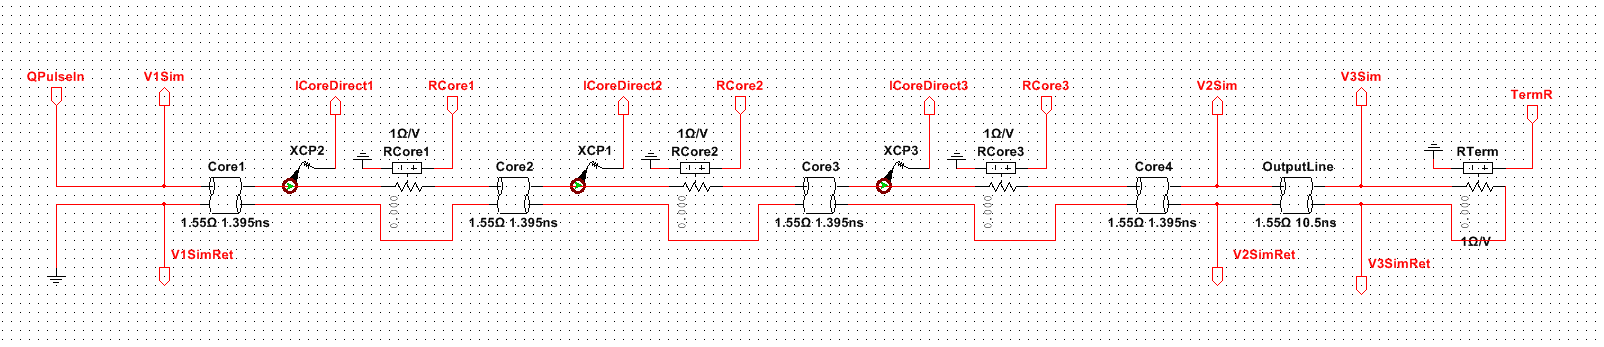
\includegraphics[scale=0.4]{image.png} 
\caption{Core Circuit Model}%
\end{center}
\end{sidewaysfigure}


\end{document}
